\question
Выпишите и/или отметьте на самом графе:
\begin{enumerate}
\item   матрицу смежности;
\item   матрицу инцидентности;
\item   список смежности;
\item   степени вершин;
\item   точки сочленения и мосты;
\item   изолированные и висячие вершины;
\item   смежные между собой сразу 3 или 4  ребра/дуги;
\item   определите и обоснуйте тип графа (простой, (не)ориентированны, мульти, псевдо, направленный и т.п.);
\item   проверьте является ли граф: регулярным/полным/двудольным/деревом (обоснуйте свои ответы);
\end{enumerate}
\begin{figure}[h]

\begin{minipage}[h]{0.55\linewidth}
\end{minipage}
\begin{minipage}[h]{0.45\linewidth}
\center{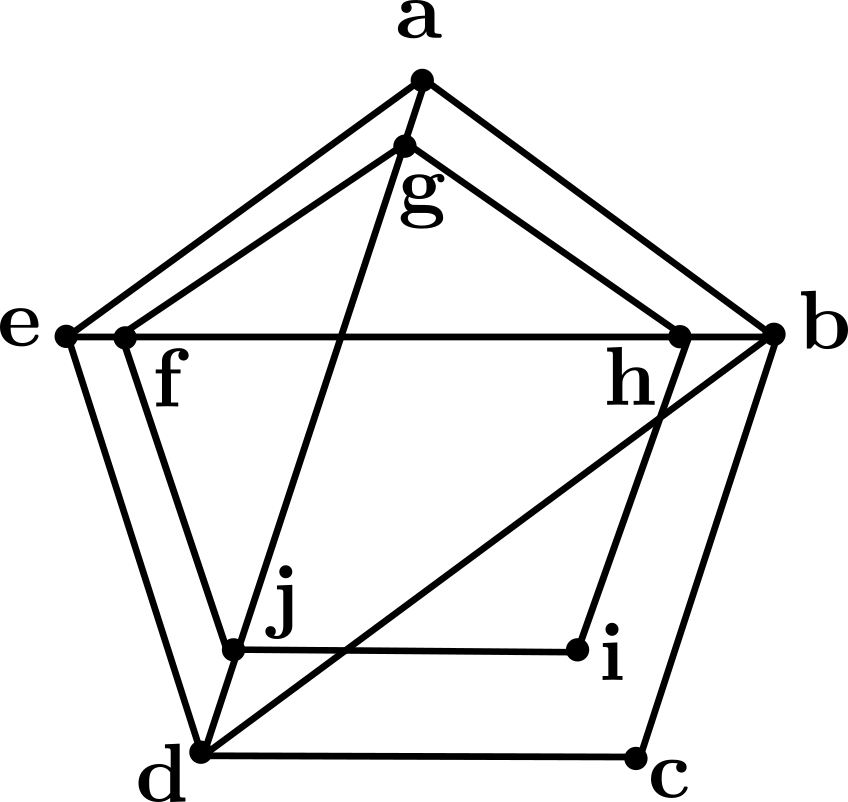
\includegraphics[width=0.5\textwidth]{pic/1.png}}
\end{minipage}
\end{figure}
